%  ----------------------------------------------------------------------------
%
%       Copyright (for the thesis) 2009 by [author - insert yourself]
%
%       This thesis is published under the
%       Creative Commons Attribution-No Derivative Works 3.0 Austria License
%       as detailed at http://creativecommons.org/licenses/by-nd/3.0/at/
%
%  ----------------------------------------------------------------------------
%  Template credits and license:
%  ----------------------------------------------------------------------------
%
%       "Fakultät für Informatik" diploma/master thesis template 2008
%
%       based upon "Diploma thesis template 2005" by lukas.silberbauer(at)gmx.at
%       based upon "Diplomarbeit mit LaTeX" by Tobias Erbsland
%       incorporating a title page by Informatik-Forum user "Baby"
%       polished and ported to the TU fonts package by Jakob Petsovits
%
%       published under the terms of
%
%  ----------------------------------------------------------------------------
%  "THE BEER-WARE LICENSE":
%  <lukas.silberbauer(at)gmx.at> wrote this file. As long as you retain this
%  notice you can do whatever you want with this stuff. If we meet some day,
%  and you think this stuff is worth it, you can buy me (us) a beer in return.
%  ----------------------------------------------------------------------------
%
%  (end of template credits)
%

\chapter{Zusätzliche Abbildungen}
\advance\abovecaptionskip by -1em

\label{chap:add_fig}
Die Dreiecksangaben bei den Bildern mit nummerierten Kamerapositionen beziehen sich auf eine Sichtweite von 400, wie sie bei den Messungen benutzt wurde. Die Bilder sind mit einer Sichtweite von 1600 aufgenommen worden und könnten wesentlich mehr Dreiecke beinhalten.\bigskip


\begin{figure}[h]
 \centering
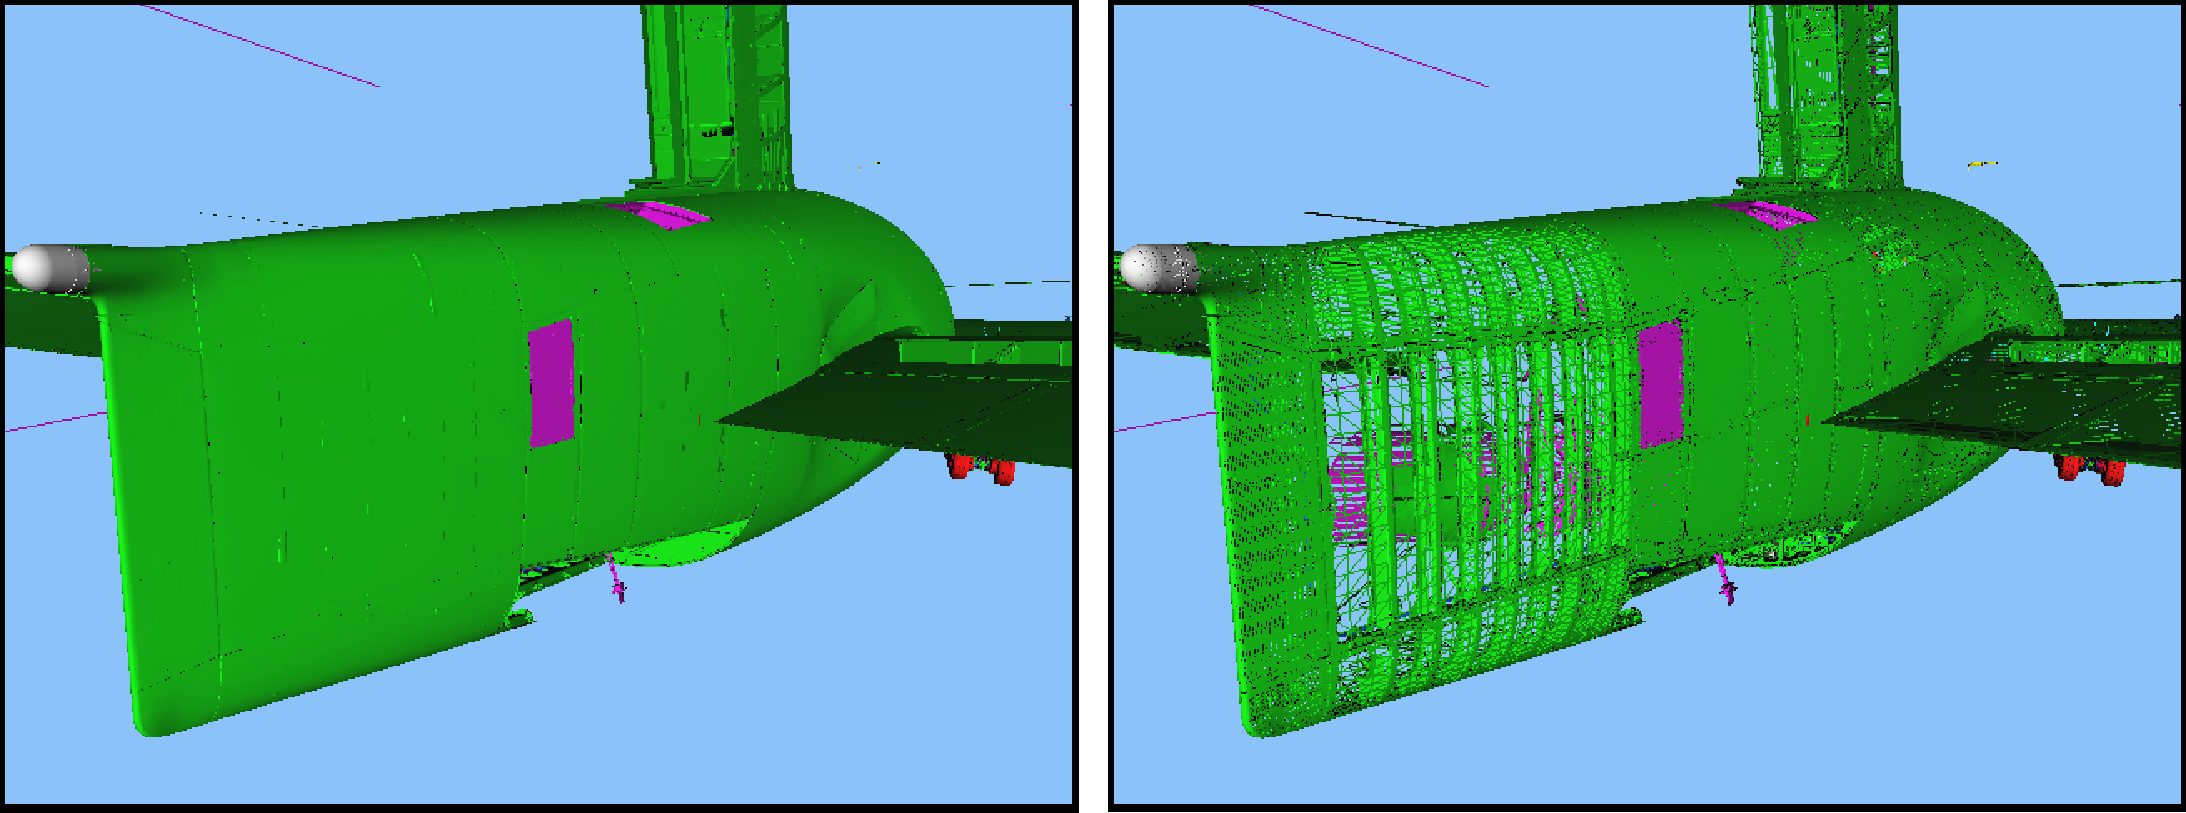
\includegraphics[width=\hsize]{images/pos1.pdf}
\caption[Kameraposition 1.]{\label{fig:eval:pos1}Kameraposition 1. (Heck außen, 3.352.475 sichtbare Dreiecke)}
\end{figure}

%\rule{\textwidth}{0.005in}

\begin{figure}[h]
\centering
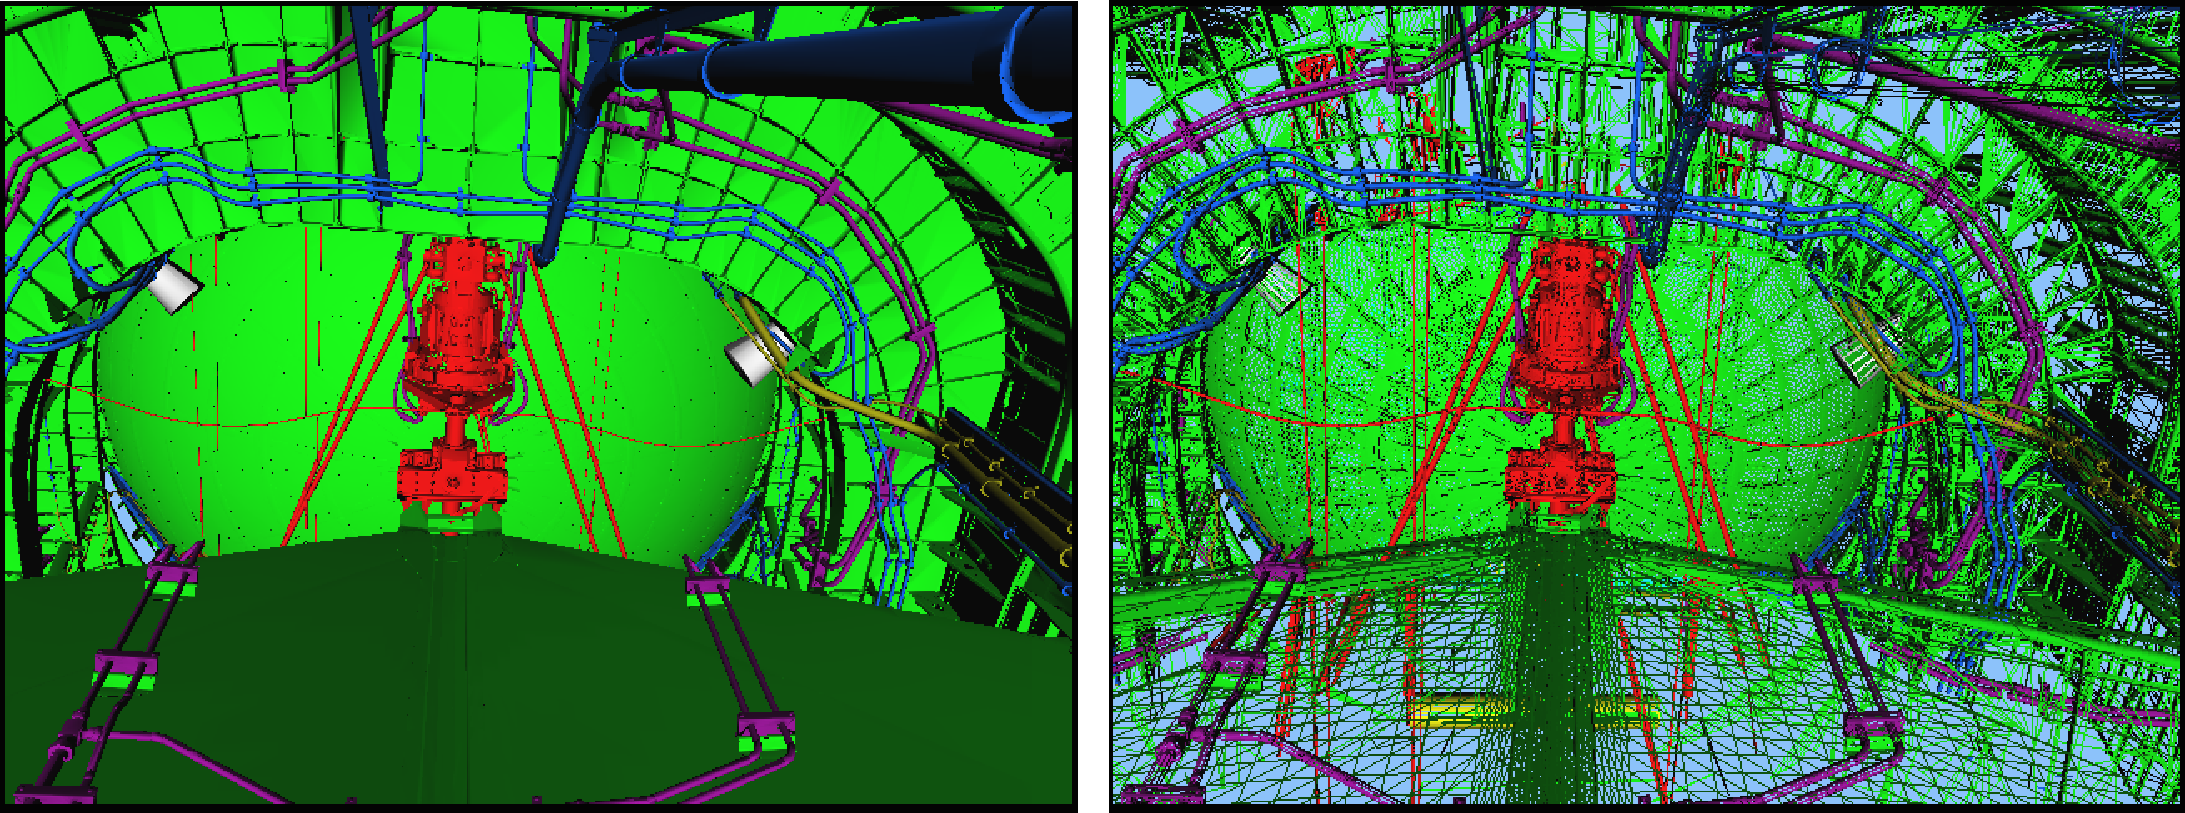
\includegraphics[width=\hsize]{images/pos2.pdf}
\caption[Kameraposition 2]{\label{fig:eval:pos2}Kameraposition 2. (Heck innen, 2.045.104 sichtbare Dreiecke)}
\end{figure}


\begin{figure}[h]
\centering
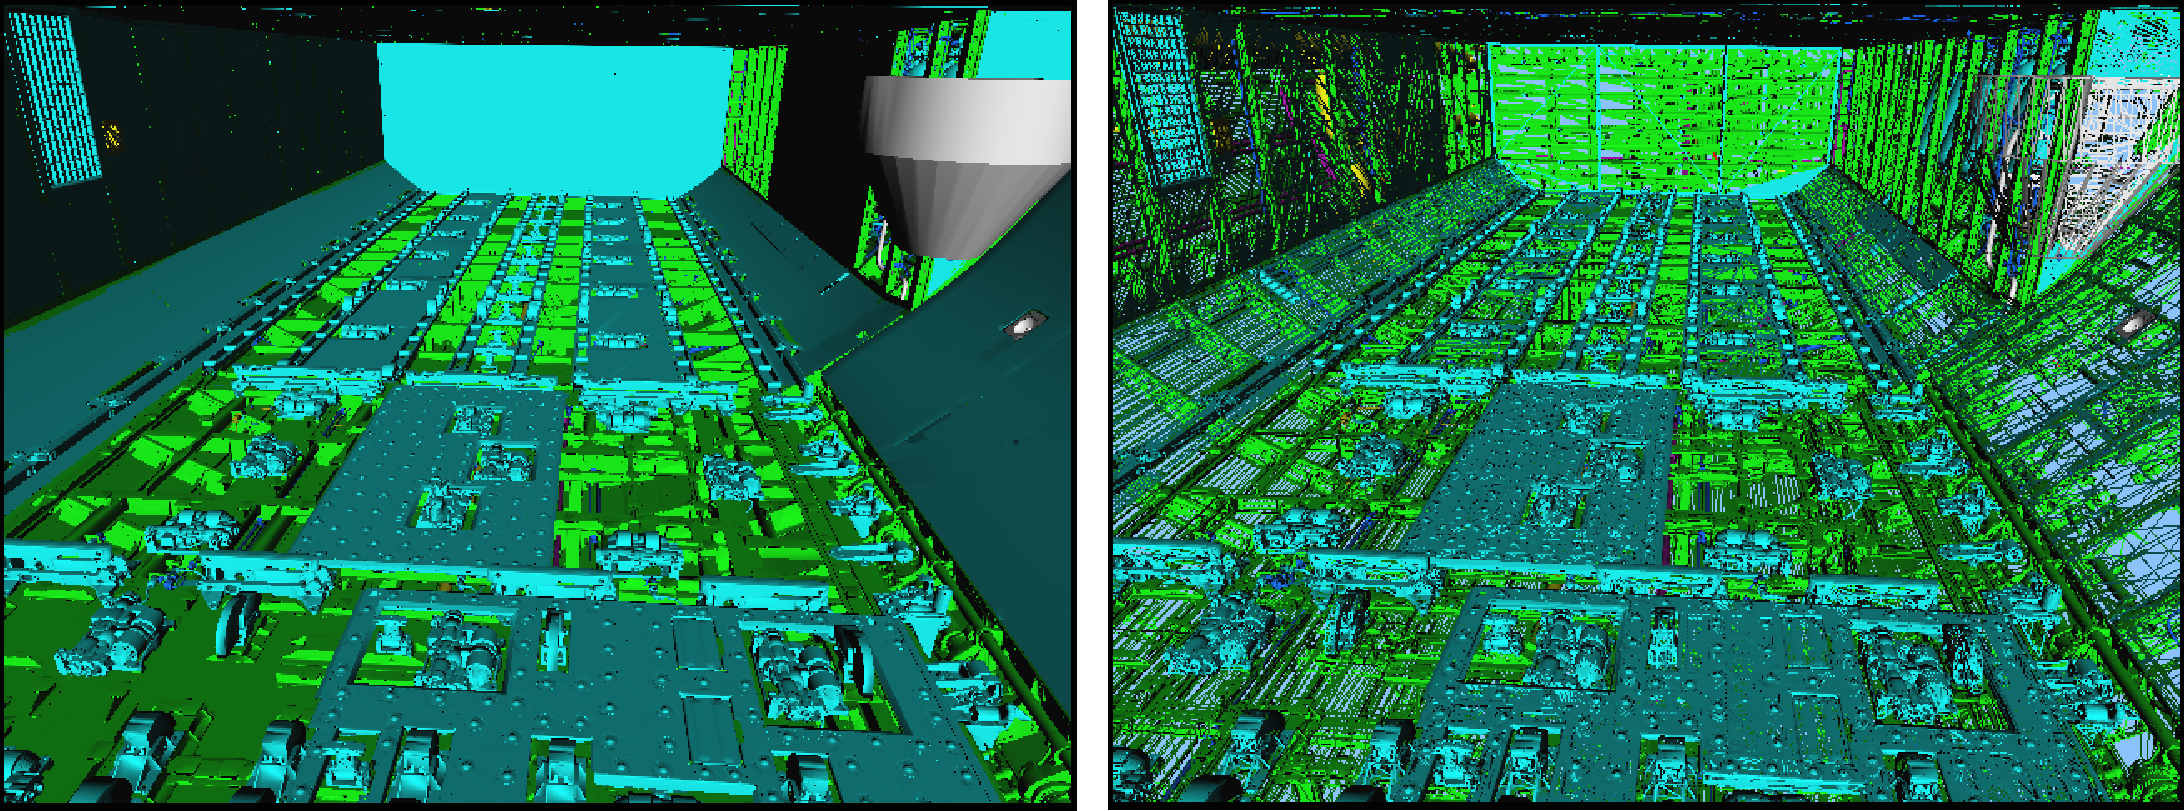
\includegraphics[width=\hsize]{images/pos4.pdf}
\caption[Kameraposition 4]{\label{fig:eval:pos4}Kameraposition 4. (Stauraum, 8.381.277 sichtbare Dreiecke)}
\end{figure}


\begin{figure}[h]
\centering
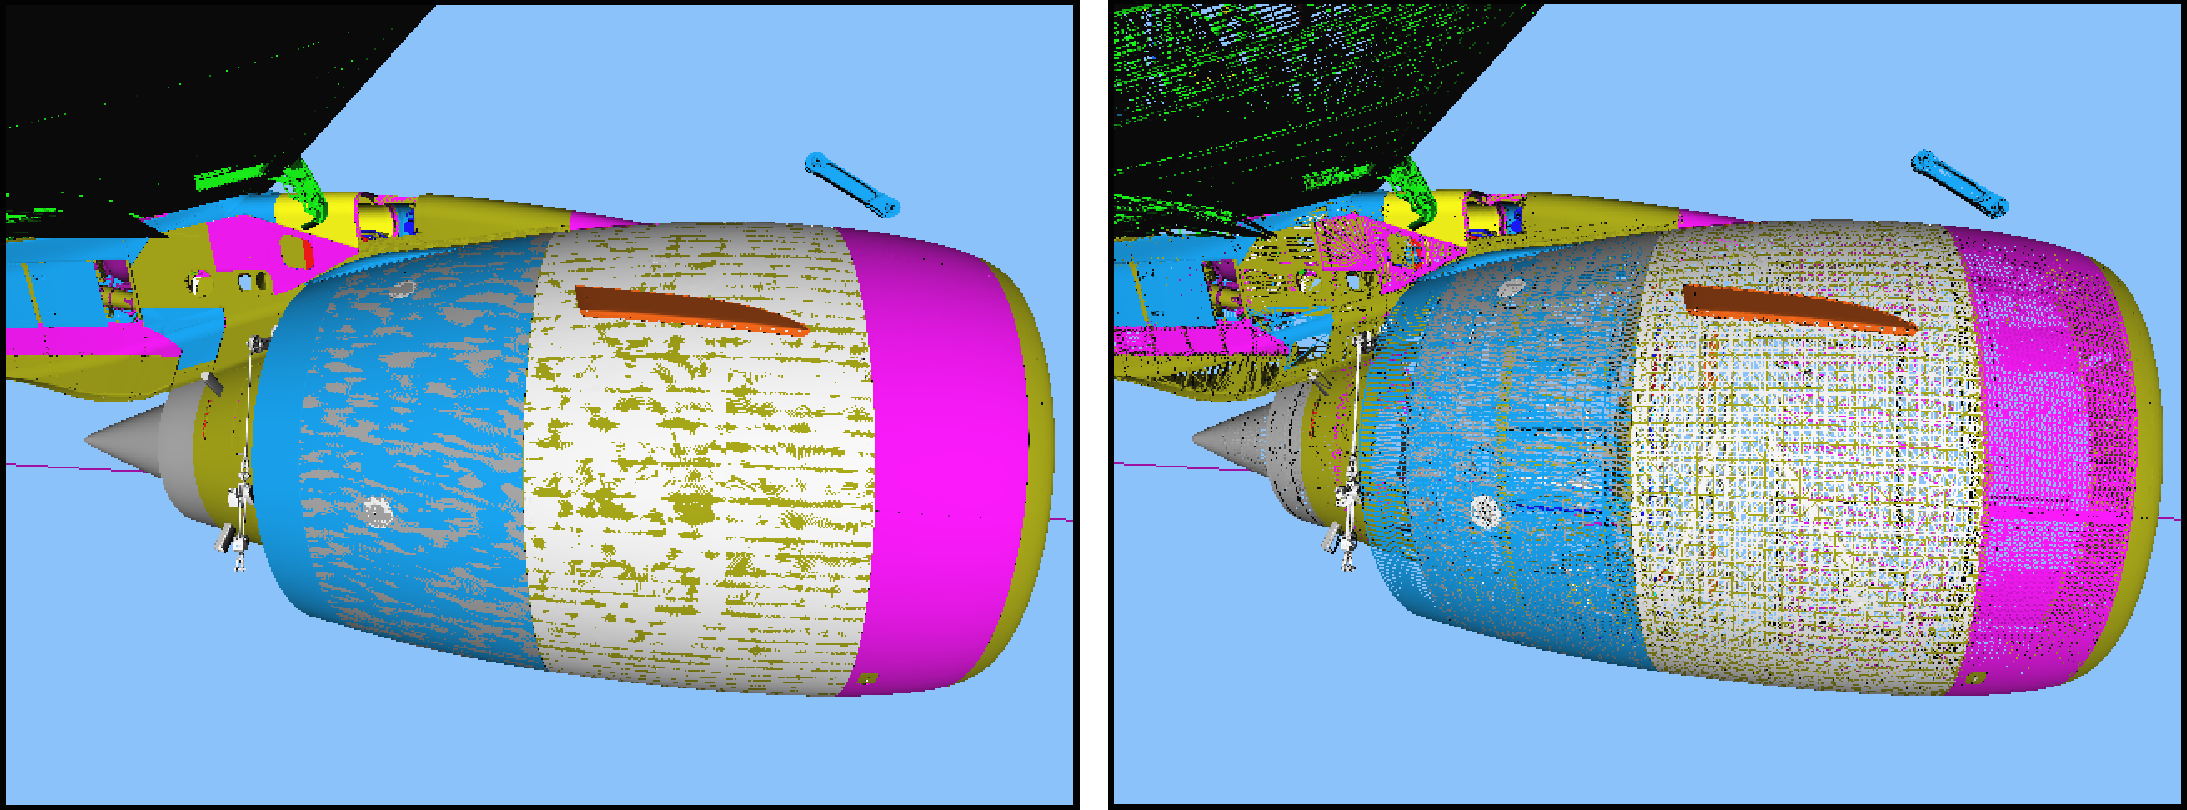
\includegraphics[width=\hsize]{images/pos6.pdf}
\caption[Kameraposition 6]{\label{fig:eval:pos6}Kameraposition 6. (Turbine, 3.381.998 sichtbare Dreiecke)}
\end{figure}


\begin{figure}
\centering
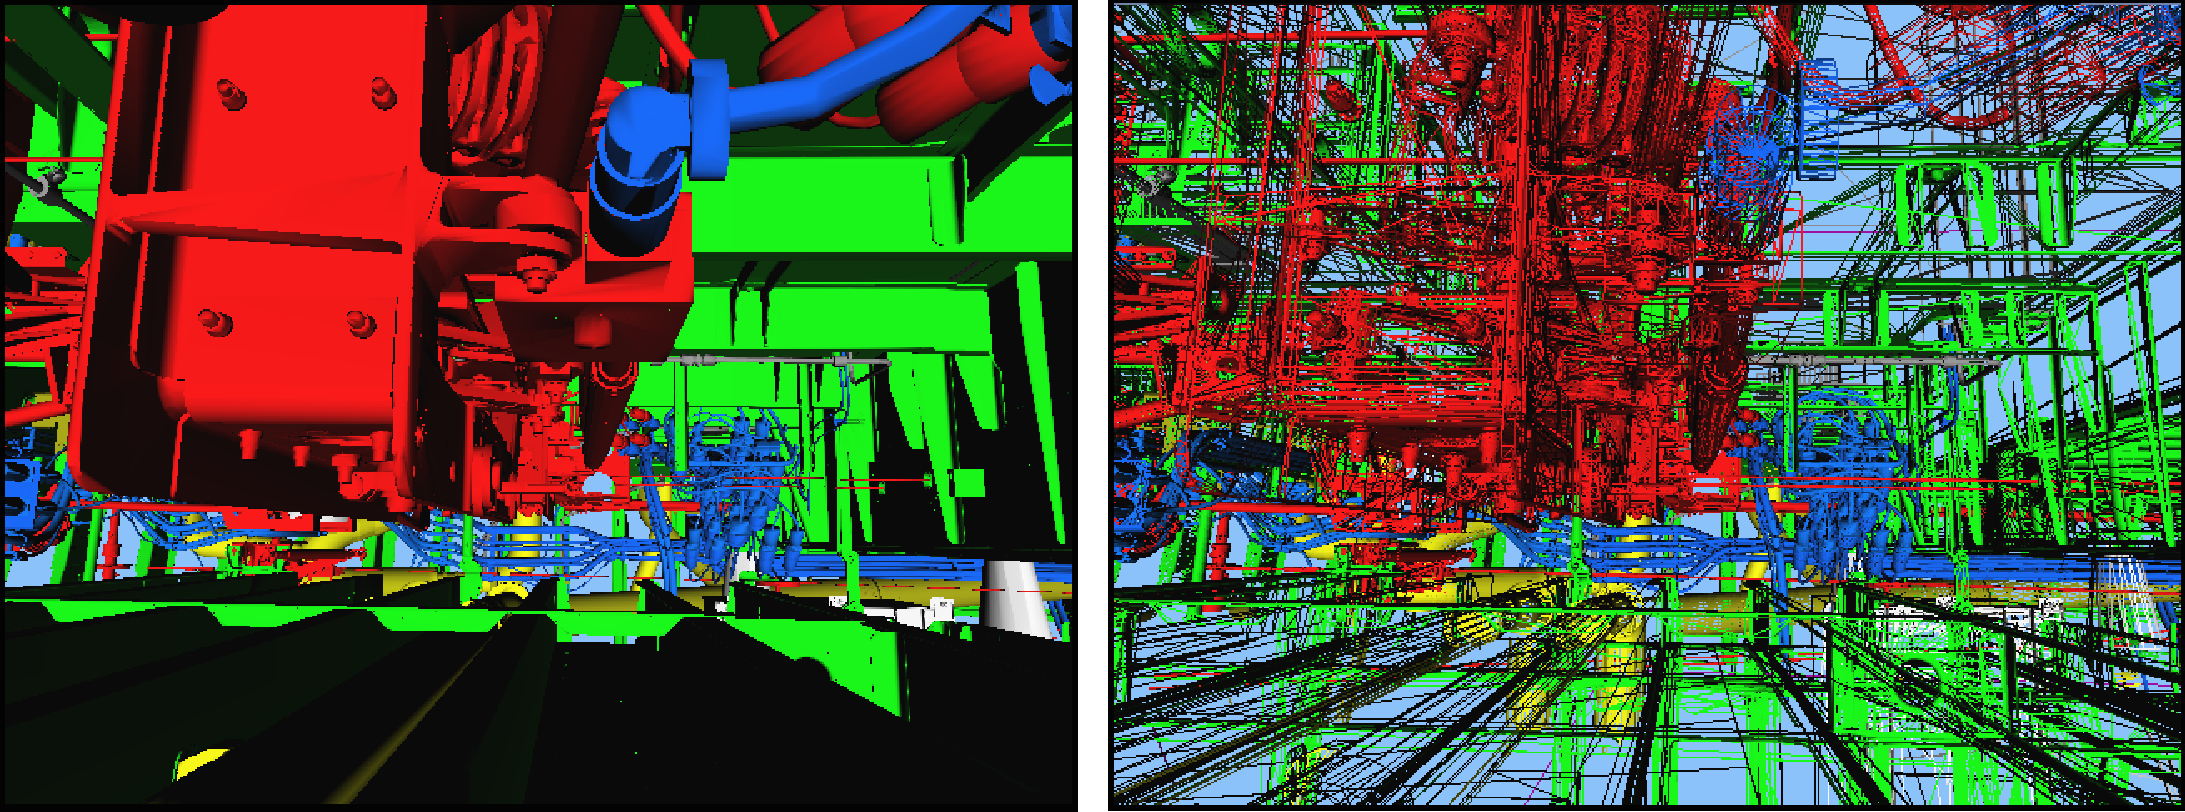
\includegraphics[width=\hsize]{images/pos7.pdf}
\caption[Kameraposition 7]{\label{fig:eval:pos7}Kameraposition 7. (Nase innen, 1.481.706 sichtbare Dreiecke)}
\end{figure}

\begin{figure}
\centering
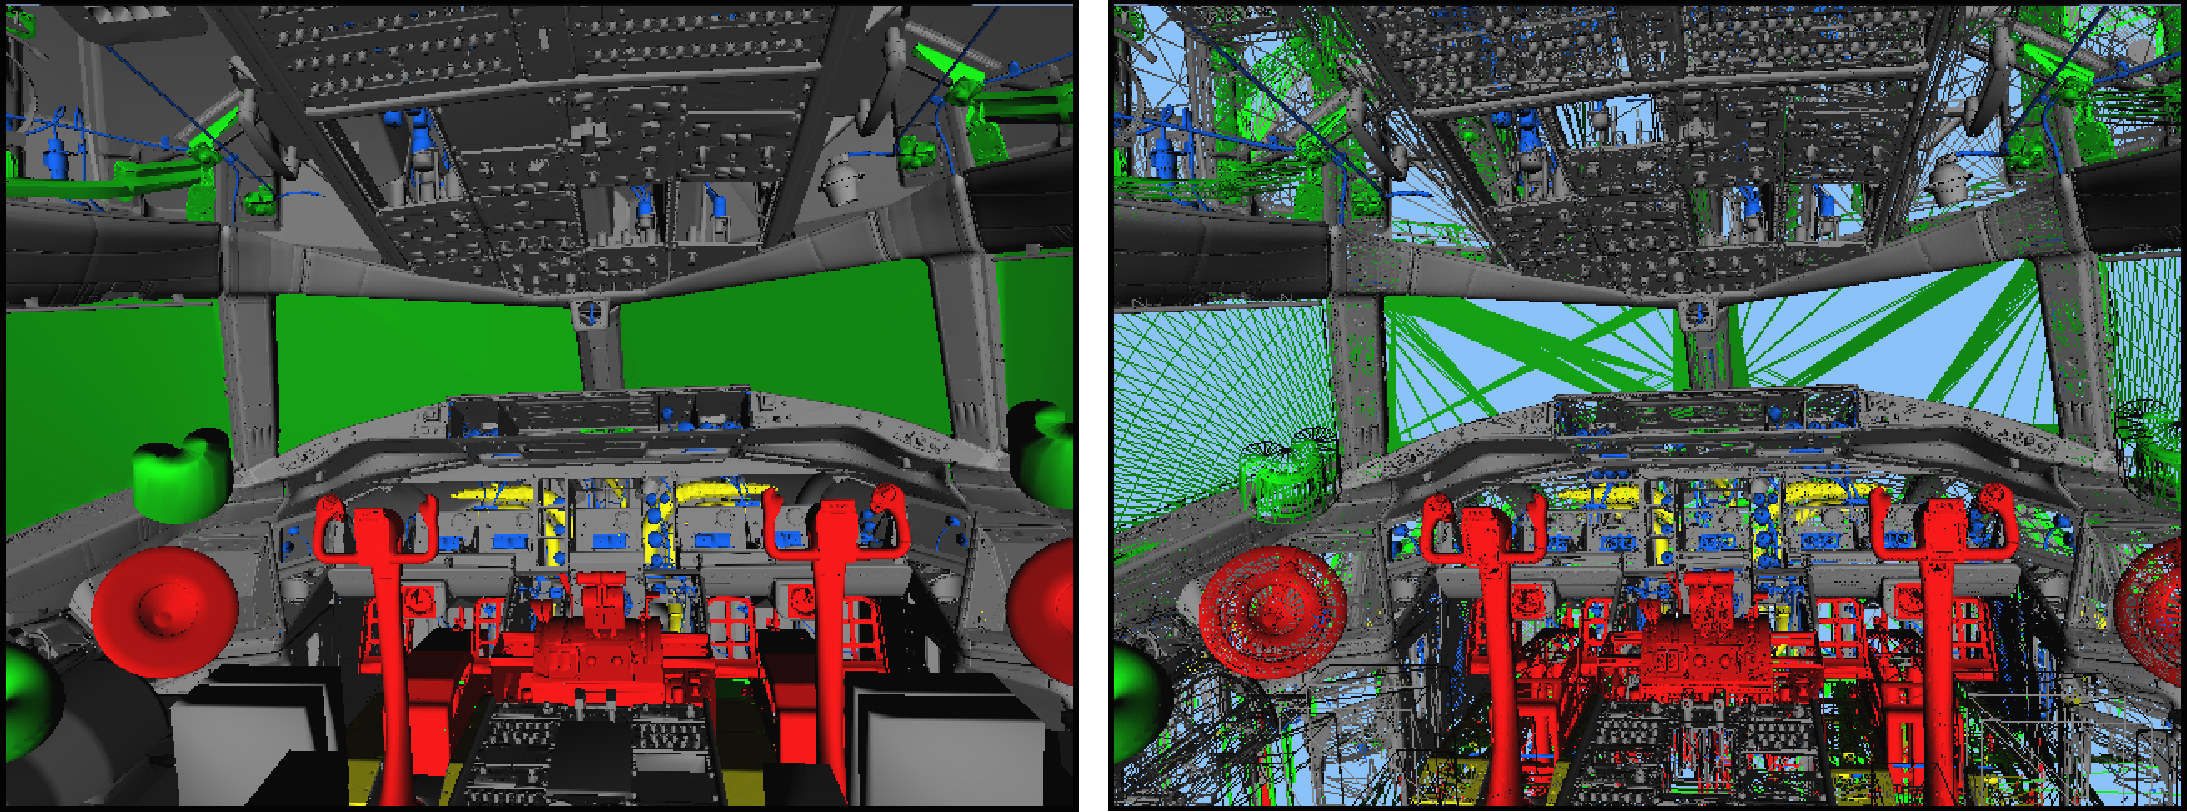
\includegraphics[width=\hsize]{images/pos8.pdf}
\caption[Kameraposition 8]{\label{fig:eval:pos8}Kameraposition 8. (Cockpit, 4.558.623 sichtbare Dreiecke)}
\end{figure}

\begin{figure}
\centering
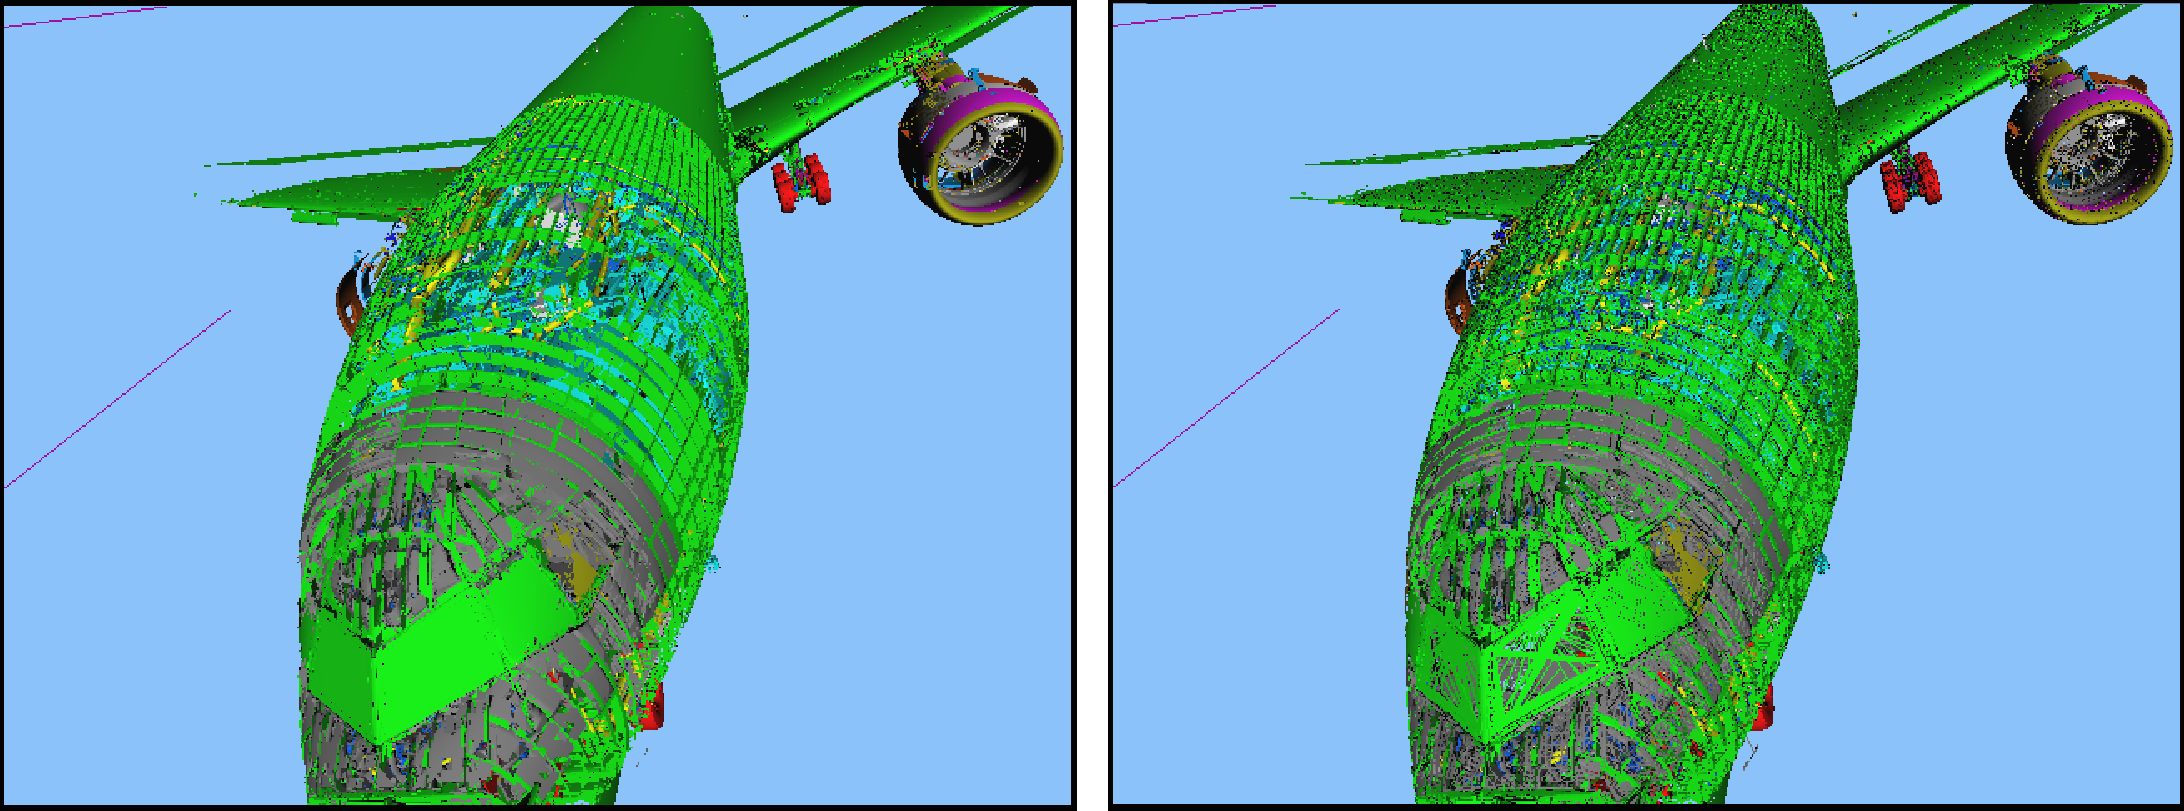
\includegraphics[width=\hsize]{images/pos9.pdf}
\caption[Kameraposition 9]{\label{fig:eval:pos9}Kameraposition 9. (Nase außen, 7.439.695 sichtbare Dreiecke)}
\end{figure}

\begin{figure}
\centering
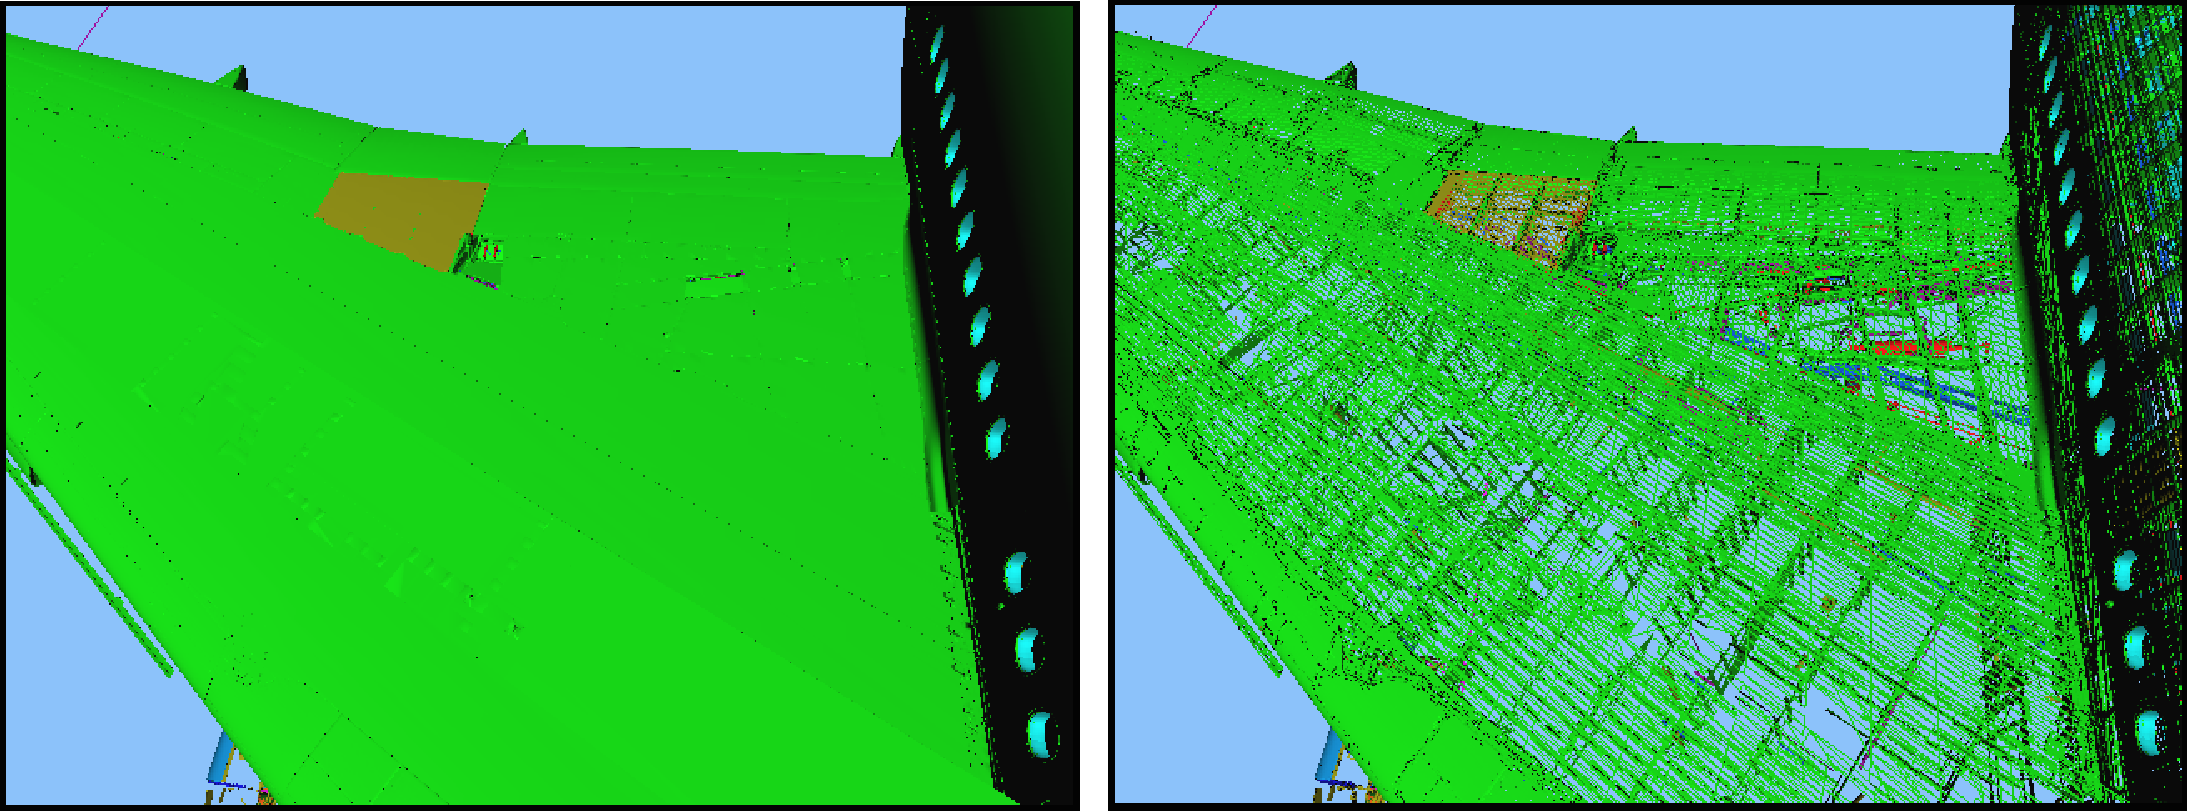
\includegraphics[width=\hsize]{images/pos10.pdf}
\caption[Kameraposition 10]{\label{fig:eval:pos10}Kameraposition 10. Flügel-Rumpf Bereich, 4.066.296 sichtbare Dreiecke)}
\end{figure}

\begin{figure}
\centering
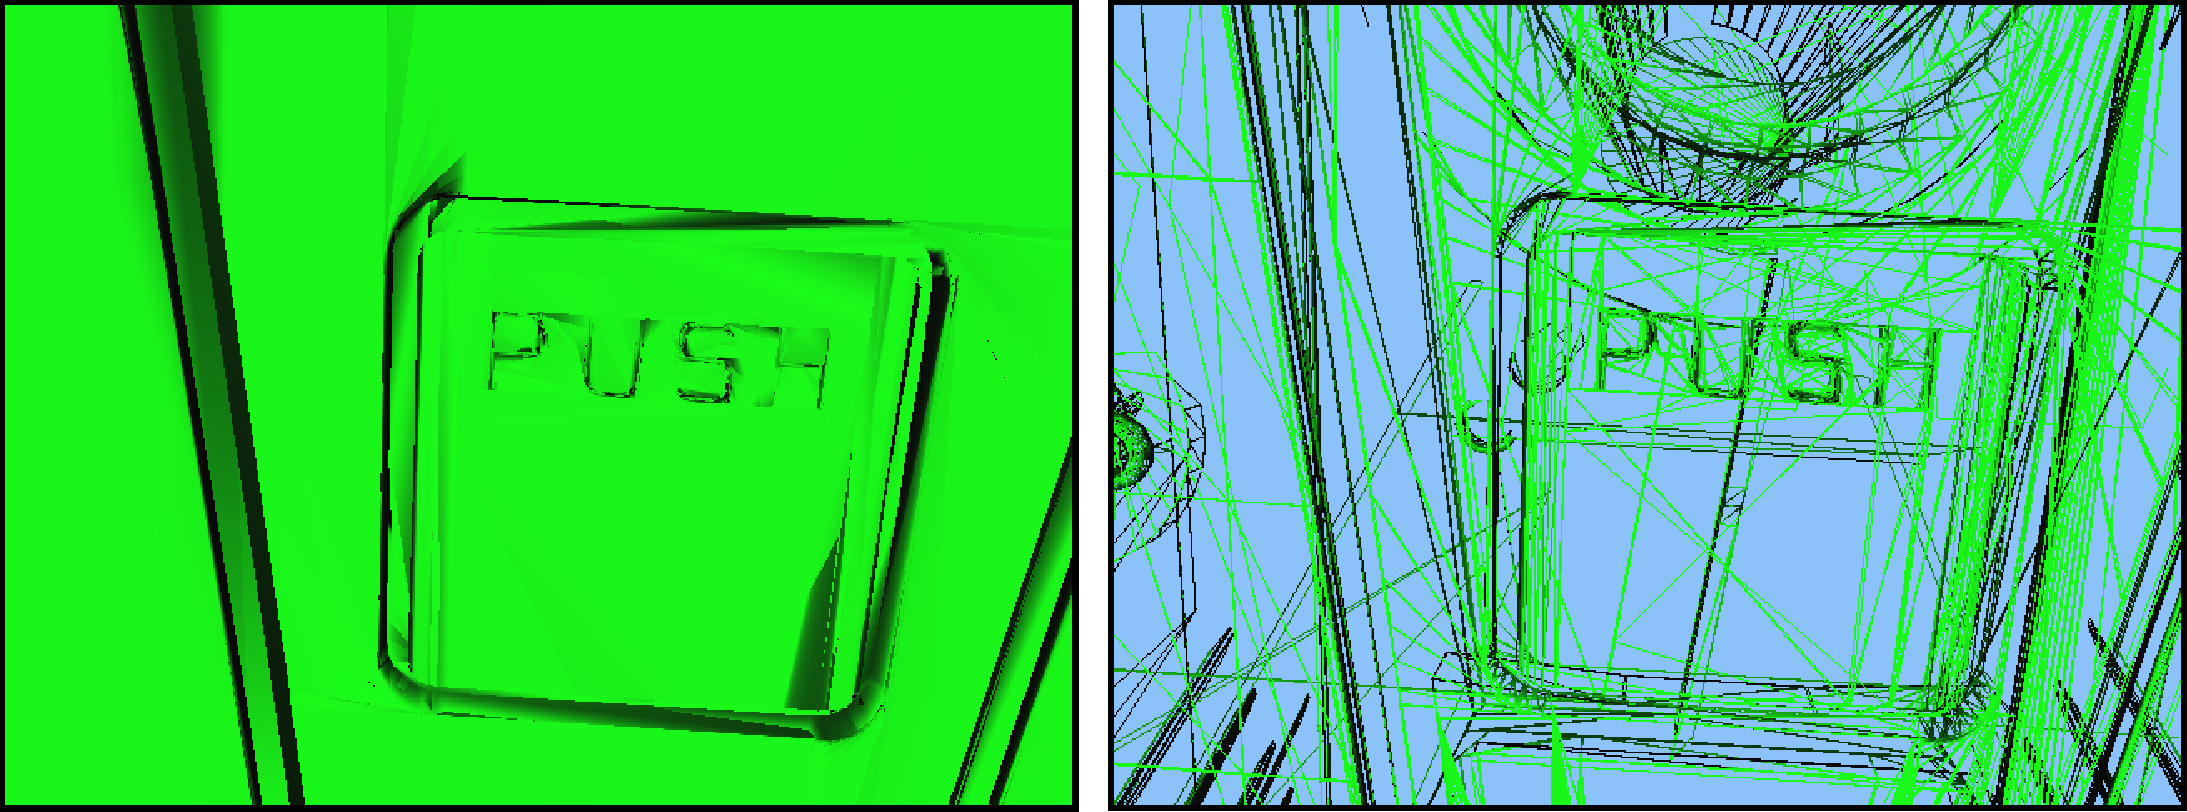
\includegraphics[width=\hsize]{images/button.pdf}
\caption{\label{fig:eval:button}Türknopf. (Bug)}
\end{figure}
\vspace{0.9cm}
\begin{figure}
\centering
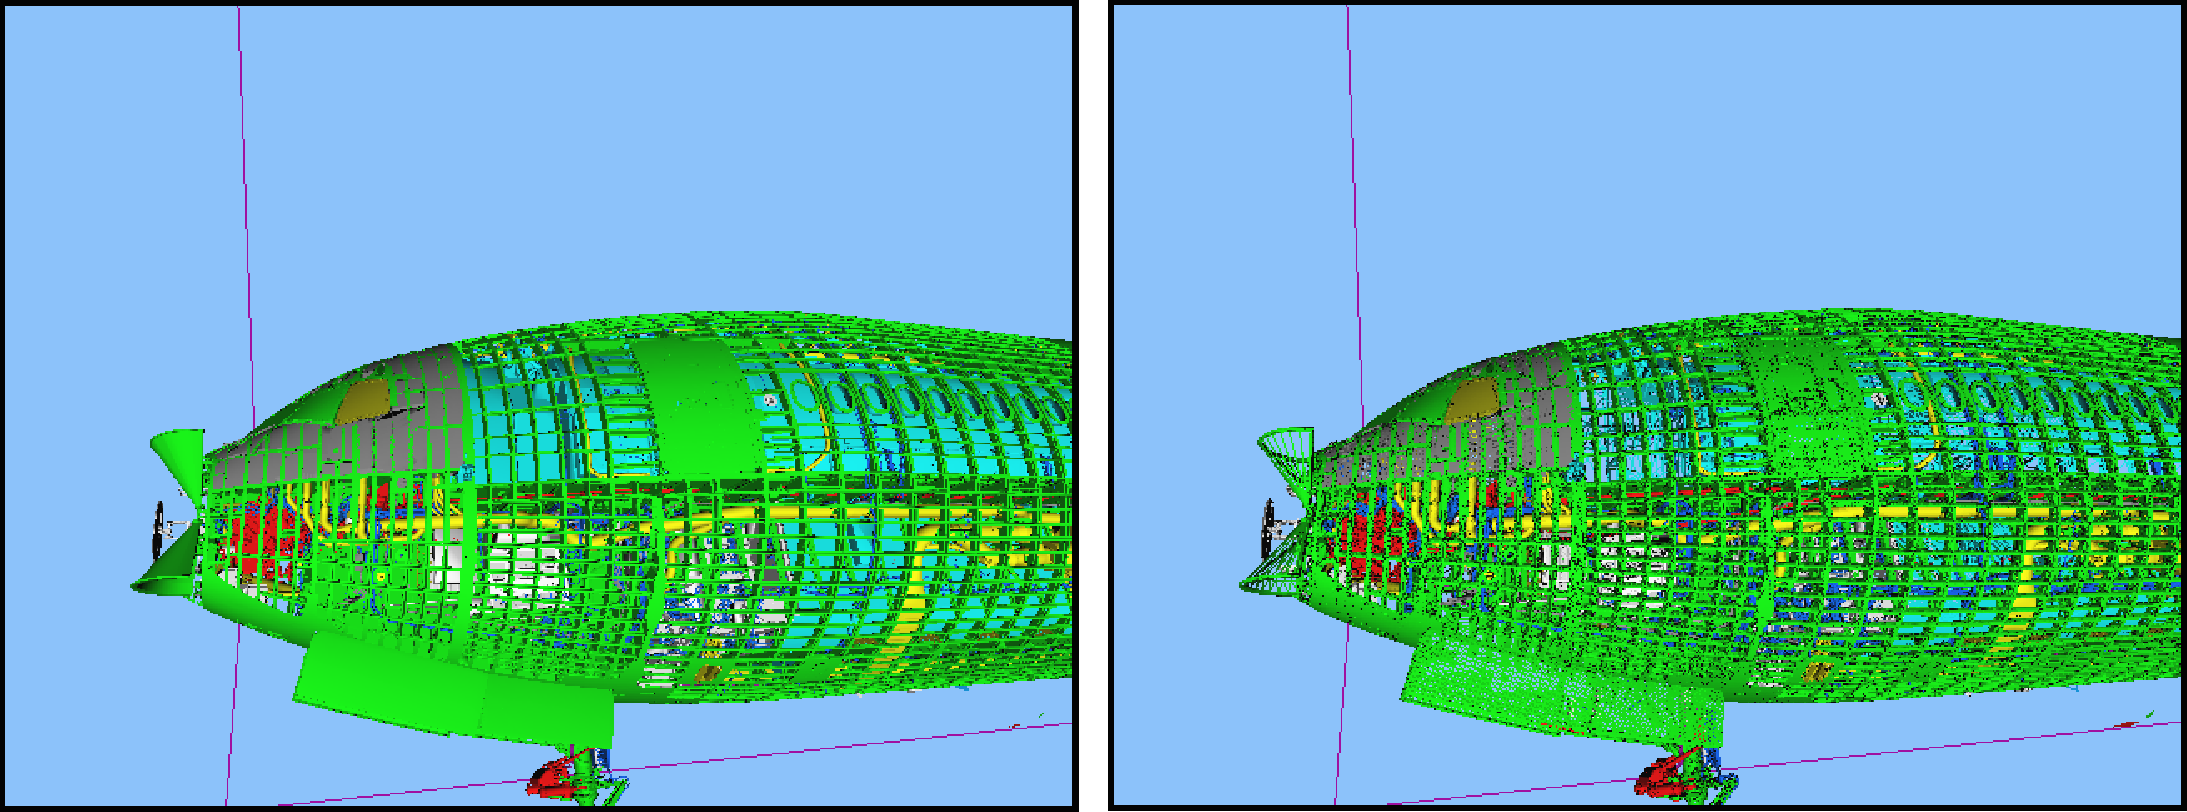
\includegraphics[width=\hsize]{images/profil_bug.pdf}
\caption{\label{fig:eval:prof_bug}Profil. (Bug)}
\end{figure}
\vspace{0.9cm}
\begin{figure}
\centering
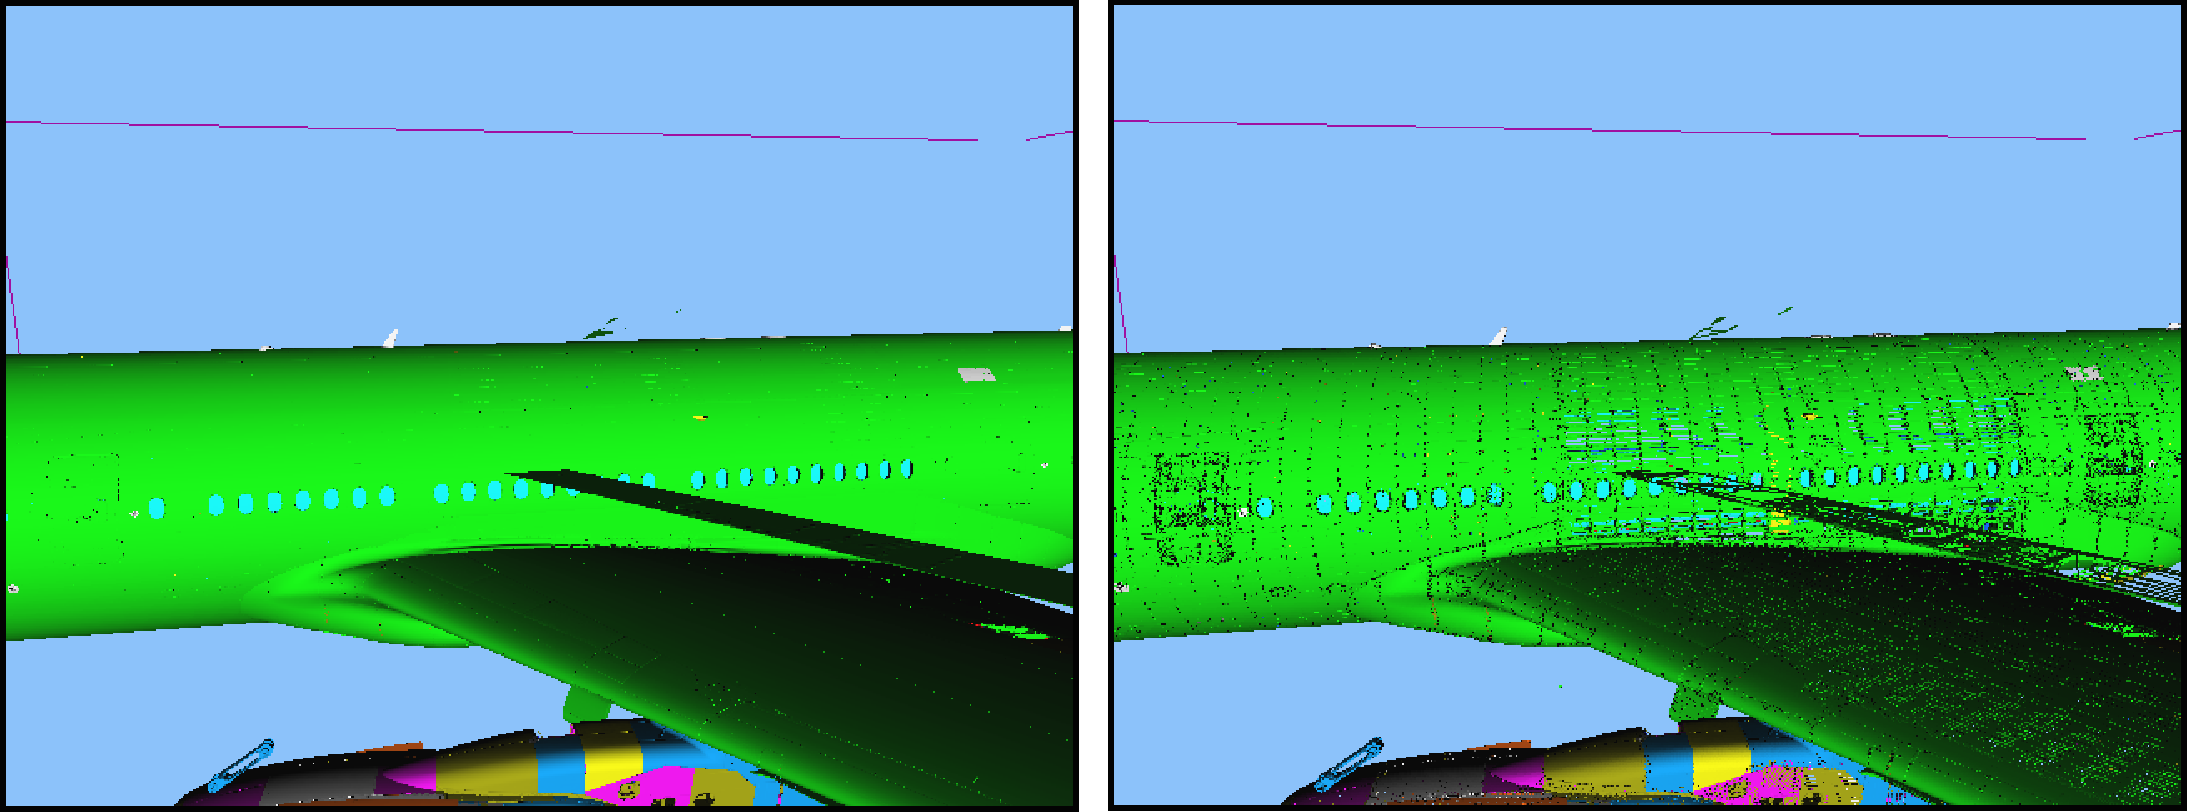
\includegraphics[width=\hsize]{images/profil_heck.pdf}
\caption{\label{fig:eval:prof_heck}Profil. (Heck)}
\end{figure}

\begin{figure}
\centering
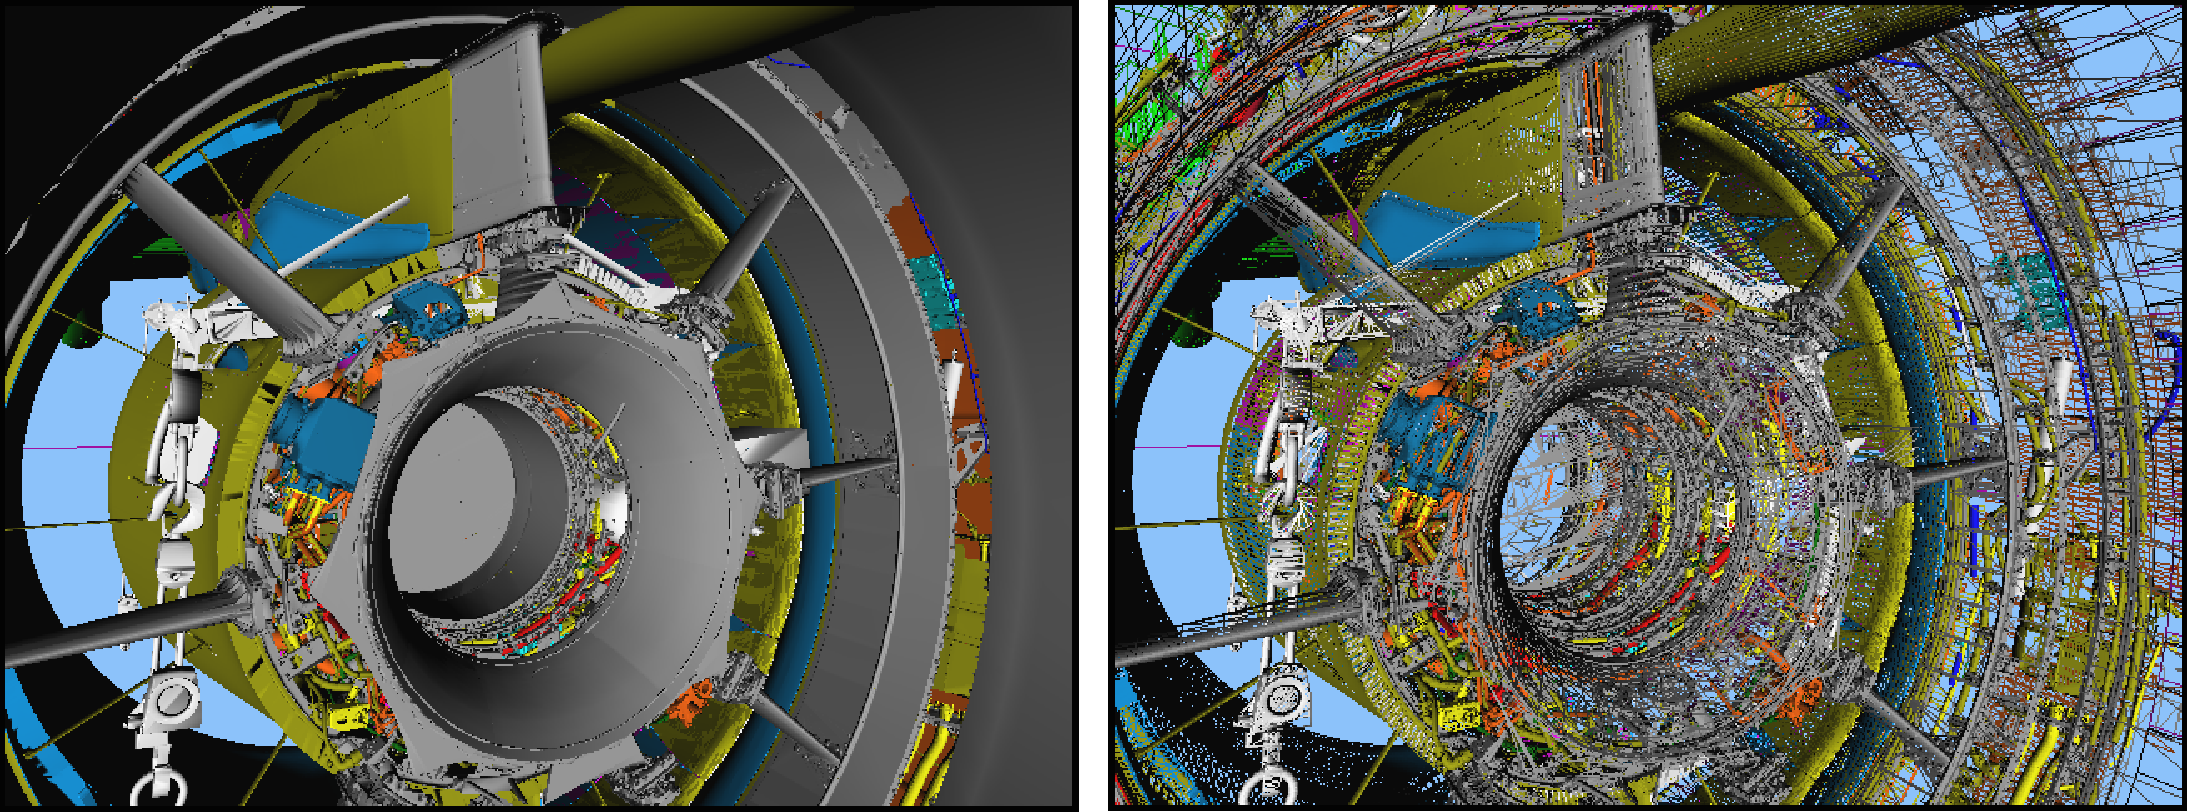
\includegraphics[width=\hsize]{images/turbine_innen.pdf}
\caption{\label{fig:eval:turbine_innen}Triebwerk 1.}
\end{figure}
\vspace{0.9cm}
\begin{figure}
\centering
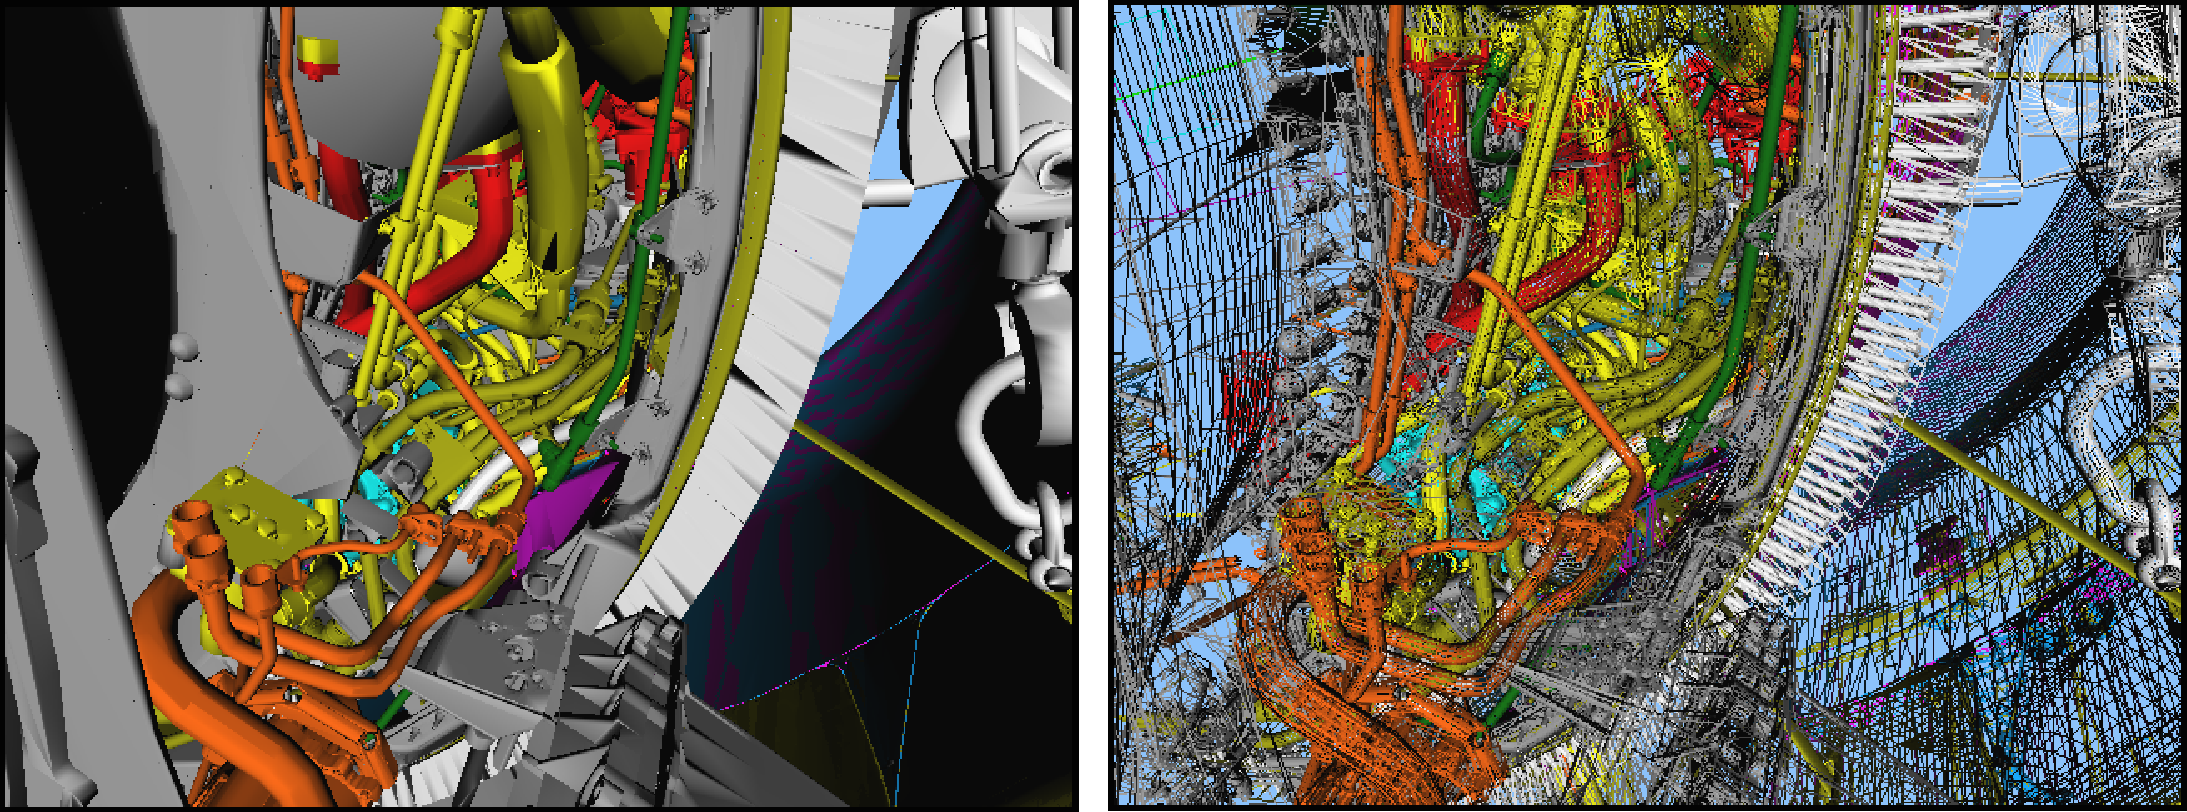
\includegraphics[width=\hsize]{images/turbine_innen2.pdf}
\caption{\label{fig:eval:turbine_innen2}Triebwerk 2.}
\end{figure}
\vspace{0.9cm}
\begin{figure}
\centering
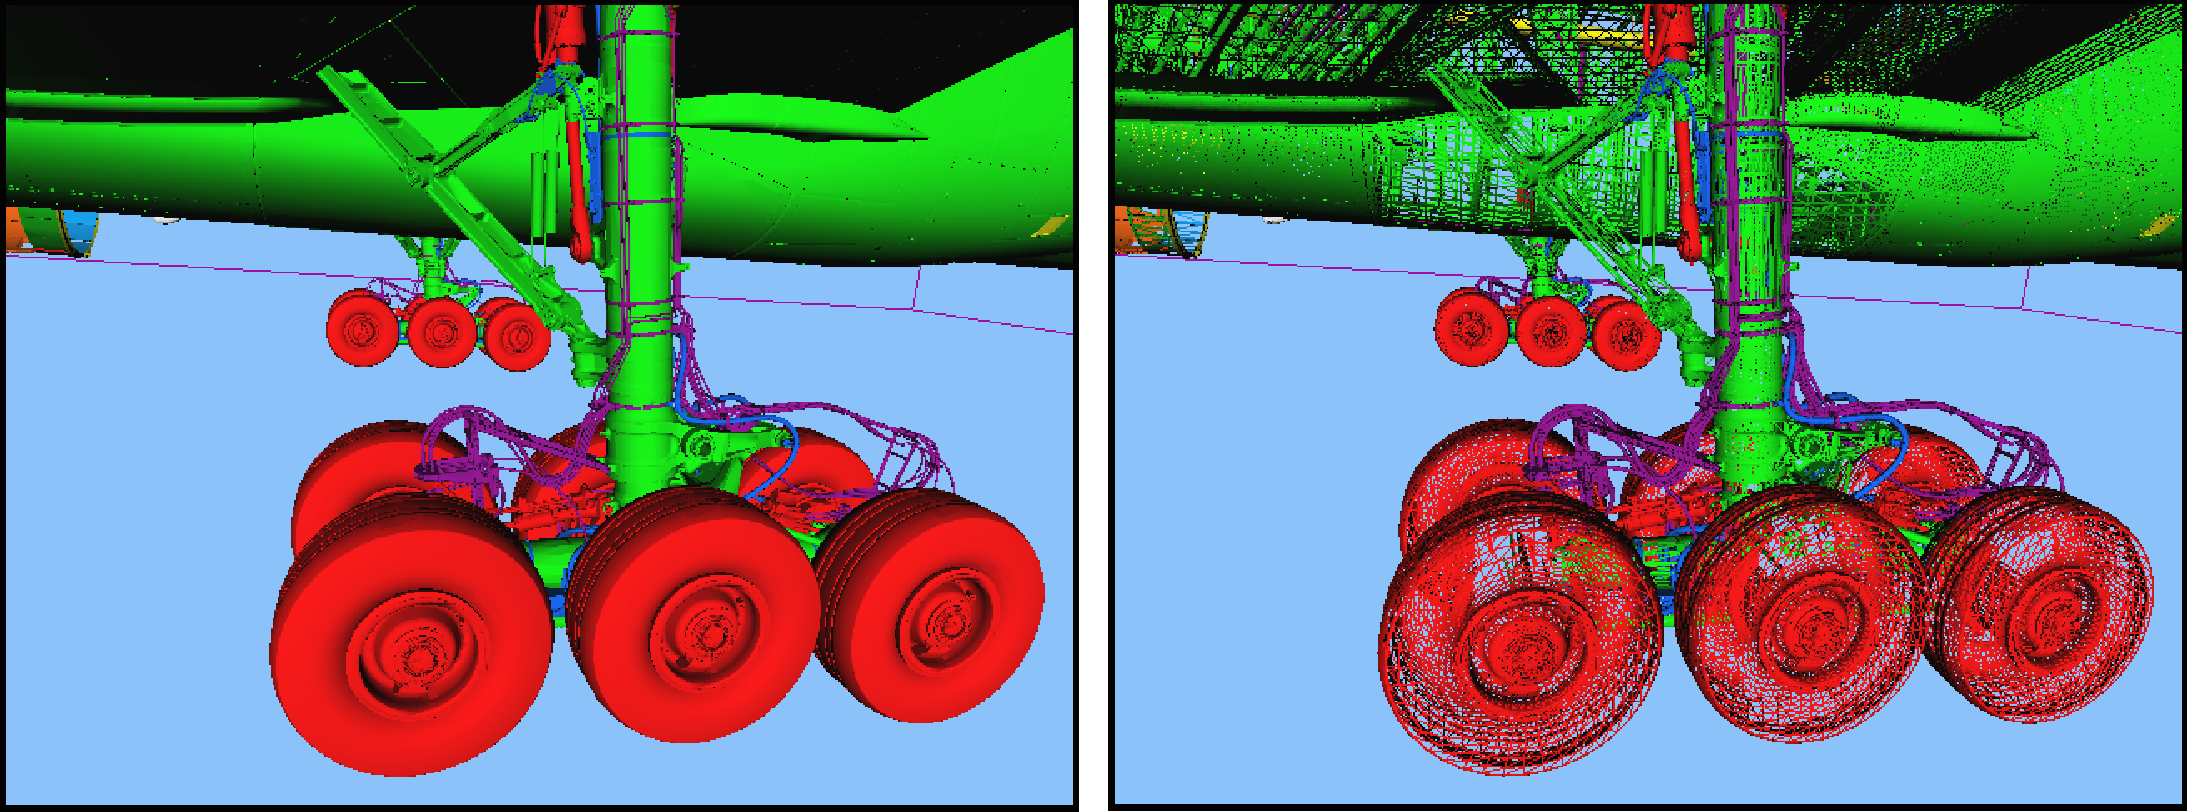
\includegraphics[width=\hsize]{images/fahrwerk.pdf}
\caption{\label{fig:eval:fahrwerk}Fahrwerk. (Heck)}
\end{figure}

%
% EOF
%
